\section{Integración de la no holonomía}
\setlength{\columnseprule}{0pt}
\twocolumn
\subsection{Error de coordenadas polares}
Error de la meta con respecto al estado actual \cite{ramirez2001control}:
\begin{equation*}
    \mathbf{z}(t) = \begin{bmatrix} a \\ \alpha \end{bmatrix}
\end{equation*}
donde:
\setlength{\overfullrule}{0pt}
\begin{align*}
    a &= \sqrt{x_e^2 + y_e^2} \\
    \alpha &= \arctan2(y_e, x_e) + \theta_e, \quad \alpha \in [-\pi, \pi]
\end{align*}
\setlength{\overfullrule}{1mm}

% Mismo reveal que la diapositiva anterior: comparte el número de figura.
\addtocounter{figure}{-1}
\begin{figure}[H]
    \centering
    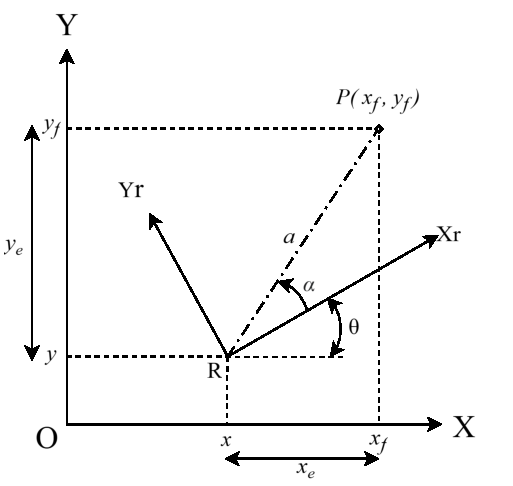
\includegraphics[width=0.9\linewidth]{Pics/error_construccion.pdf}
    \caption{Definición del error}
    \label{fig:error_coords_polares}
\end{figure}
